\documentclass[a4paper,12pt]{article}
%%%%%~~~~~~~~~~~~~~~~~~~~~usepackage~~~~~~~~~~~~~~~~~
\usepackage{rotating}
\usepackage[top=1in, bottom=1in, left=1in, right=1in]{geometry}
\usepackage{graphicx}
\usepackage[numbers,square,sort&compress]{natbib}
\usepackage{setspace}
\usepackage[cdot,mediumqspace,]{SIunits}
\usepackage{caption}
\usepackage{subcaption}
\usepackage{mathtools}
\usepackage{authblk}
\usepackage{float}

%%%%%%~~~~~~~~~~~~~~~new command~~~~~~~~~~~~~~~~~~~~

\newcommand{\myemail}{ayushi.singh@mail.utoronto.ca}

%%%%%%%%~~~~~~~~~Title and etc~~~~~~~~~~~~~~~~~~~~~~~~~

\begin{document}
\onehalfspacing
\title{Photon Counting and the Statistics of Light}
\author{Ayushi Singh, Anita Bahmanyar, Carly Berard}
%\affil{{\myemail}, University of Toronto, ON}
\date{30 September, 2013}
\maketitle
%\altaffiltext{1}{{\myemail}}
%\altaffilmark{1}
%%%%%%%%%%%~~~~~~~~~~~~~~~~Abstract~~~~~~~~~~~~~~~
\begin{abstract}
\label{abstract}
Write the abstract about the experiment where we are collecting particles using PMT, analyzing it's distribution and comparing it with theoretical prediction. We are also taking the errors and using python to get count rate, mean and standard Deviation.
\end{abstract}

%%%%%%~~~~~~~~~~~~Introduction
\section{Introduction}
\label{sec:introduction}

%%%%%%~~~~~~~~~~~~Equipment
\section{Equipment}
\label{sec:equipment}

%%%%%%%~~~~~~~~~~~~Procedure
\section{Procedure}
\label{sec:procedure}

%%%%%%%%%%~~~~~~~~~~Data
\section{Data Summary}
\label{sec:data}

%%%%%%%%%~~~~~~~~~~~Discussion
\section{Discussion}
\label{sec:diccussion}

%%%%%%%~~~~~~~ light
\subsection{Variation in light count} 
\label{sec:light}

%#################################################
\begin{figure}[H]
\centering
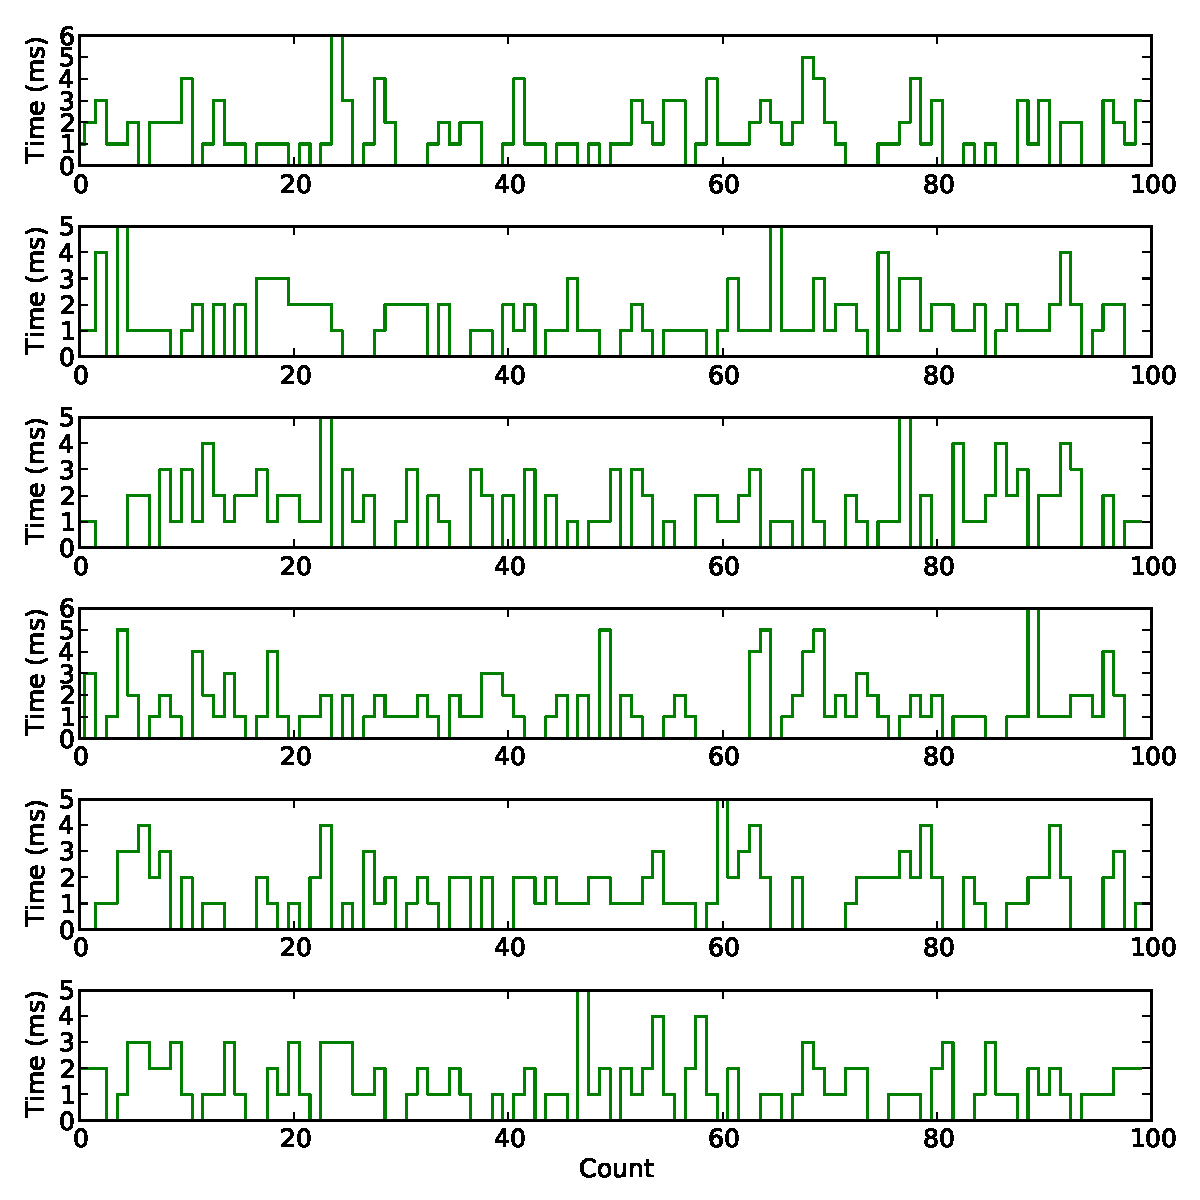
\includegraphics[angle=0,height=12cm,width=15.5cm]{graphs/task1.pdf}
\caption{Count per Sample vs. Time graph for six set of data, where time interval of each sample is 0.001s for 100 samples}
\label{fig:task1_plots}
\end{figure}

\begin{figure}[H]
\centering
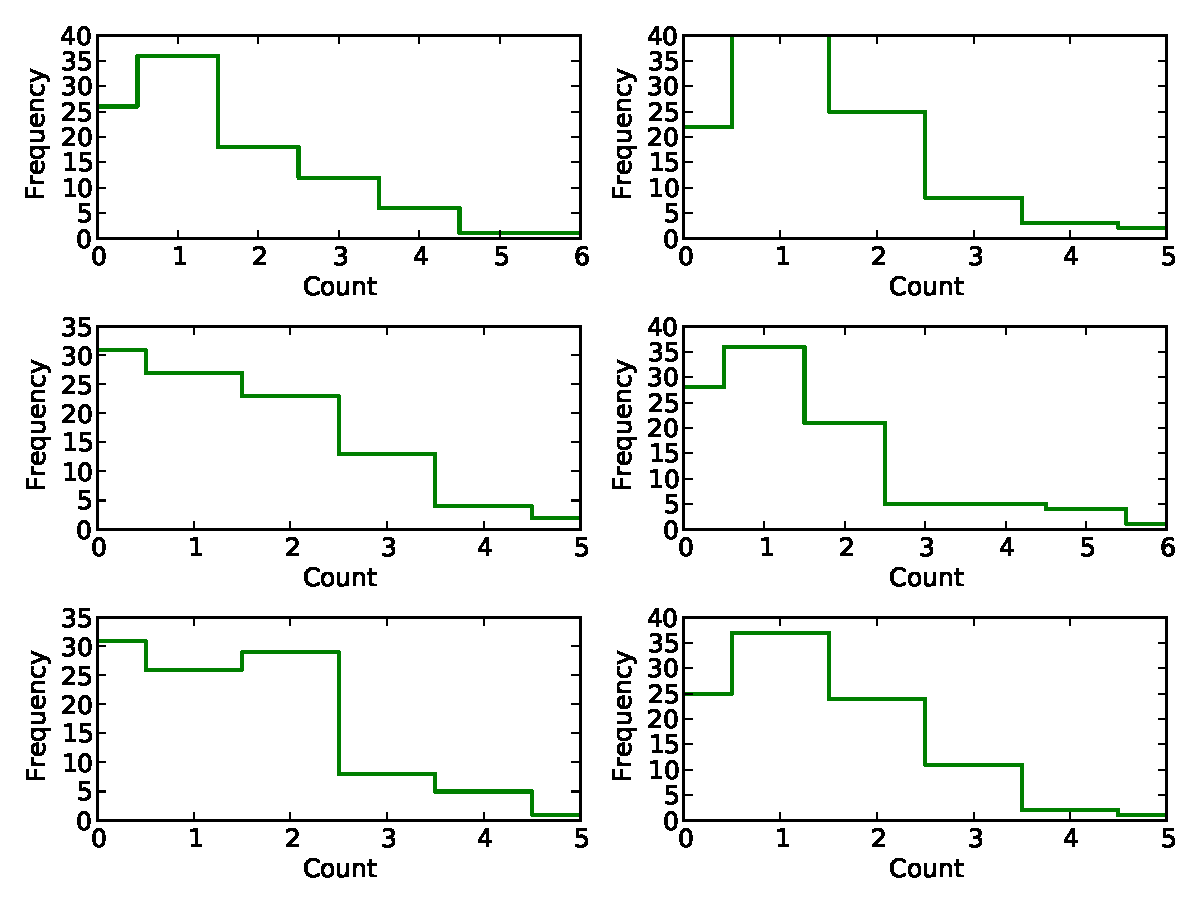
\includegraphics[angle=0,height=12cm,width=15.5cm]{graphs/task1_hist.pdf}
\caption{Histogram of data plotted in Figure \ref{fig:task1_plots}, where time interval of each sample is 0.001s for 100 samples }
\label{fig:task1_hist}
\end{figure}
%#################################################
Explain the how they are random but have similar mean and SD. And how their histogram are some what simialr but still every random
%#################################################
\begin{figure}[H]
\centering
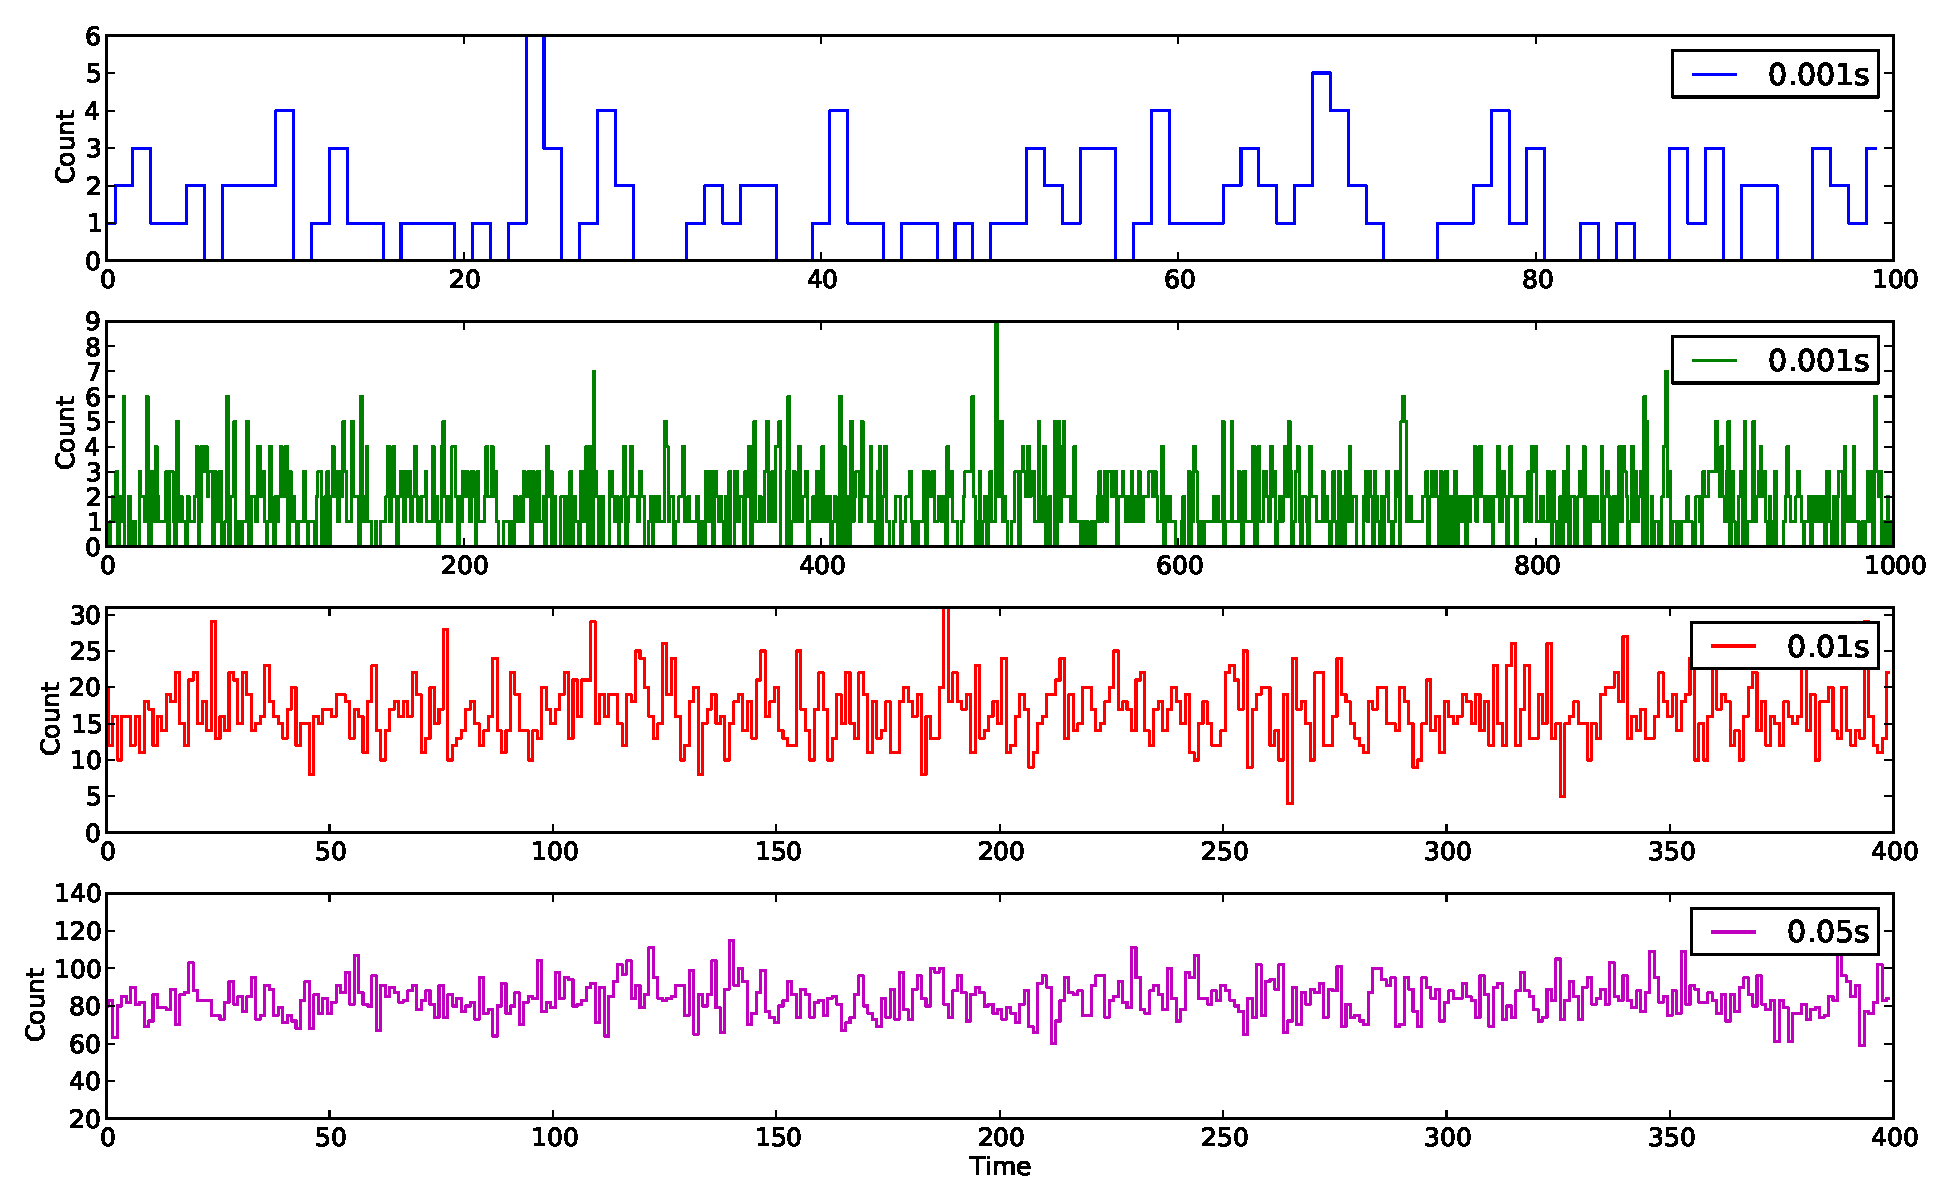
\includegraphics[angle=0,height=10cm,width=15.5cm]{graphs/diff_plots.pdf}
\caption{Count per Sample vs. Time graph for four different set of data. Blue and green graphs show affect of change in sample numbers, where as, red and margenta graphs show variation by changing time interval.}
\label{fig:diff_plot}
\end{figure}

\begin{figure}[H]
\centering
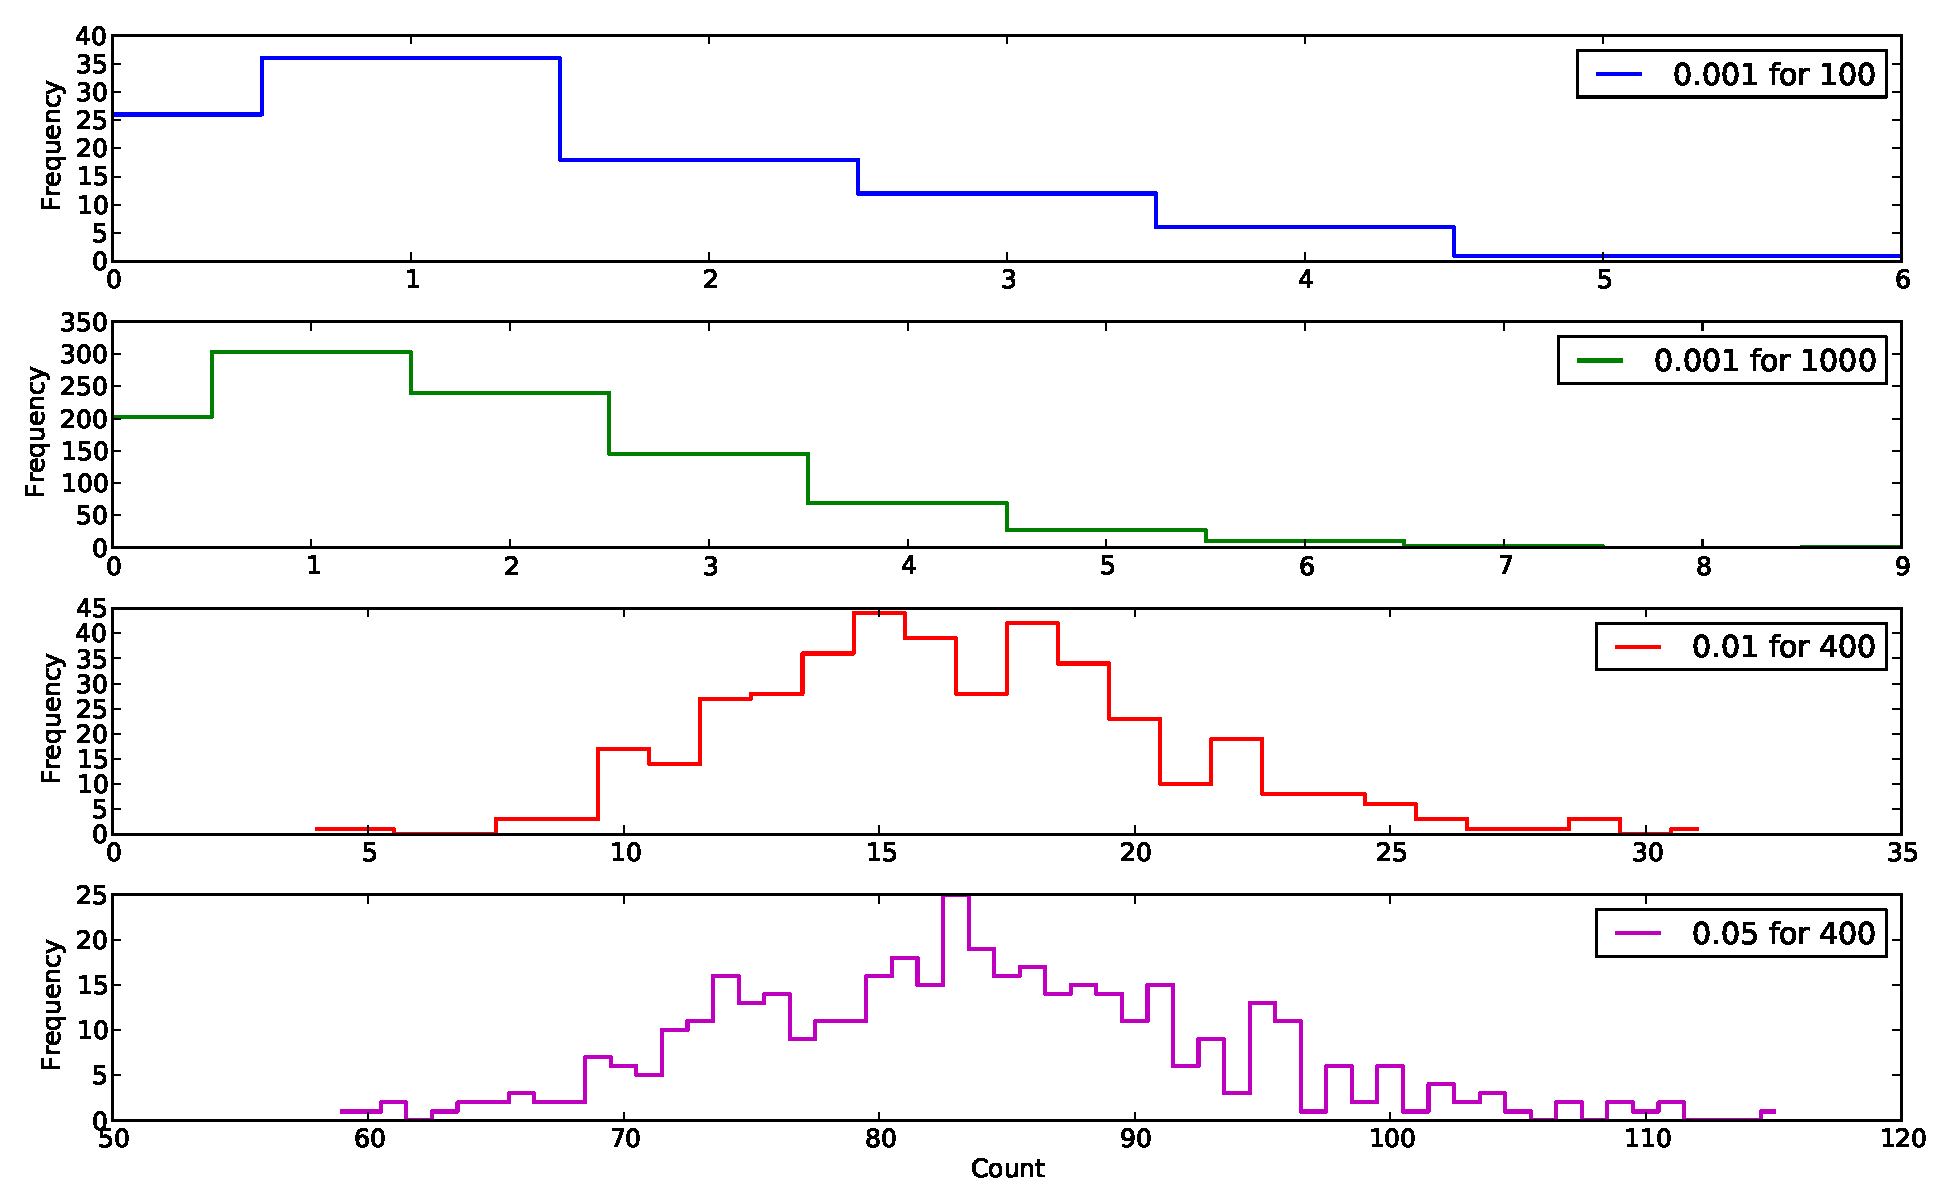
\includegraphics[angle=0,height=10cm,width=15.5cm]{graphs/diff_hist.pdf}
\caption{Histogram of data plotted in Figure \ref{fig:diff_plot}}
\label{fig:diff_hist}
\end{figure}

%#################################################

%%%%%%~~~~~~~Dark
\subsection{Effect of Dark Count}
\label{sec:dark}
Explain what is dark counts?? How Did you achive them. what is different about them
%#################################################
\begin{figure}[H]
\centering
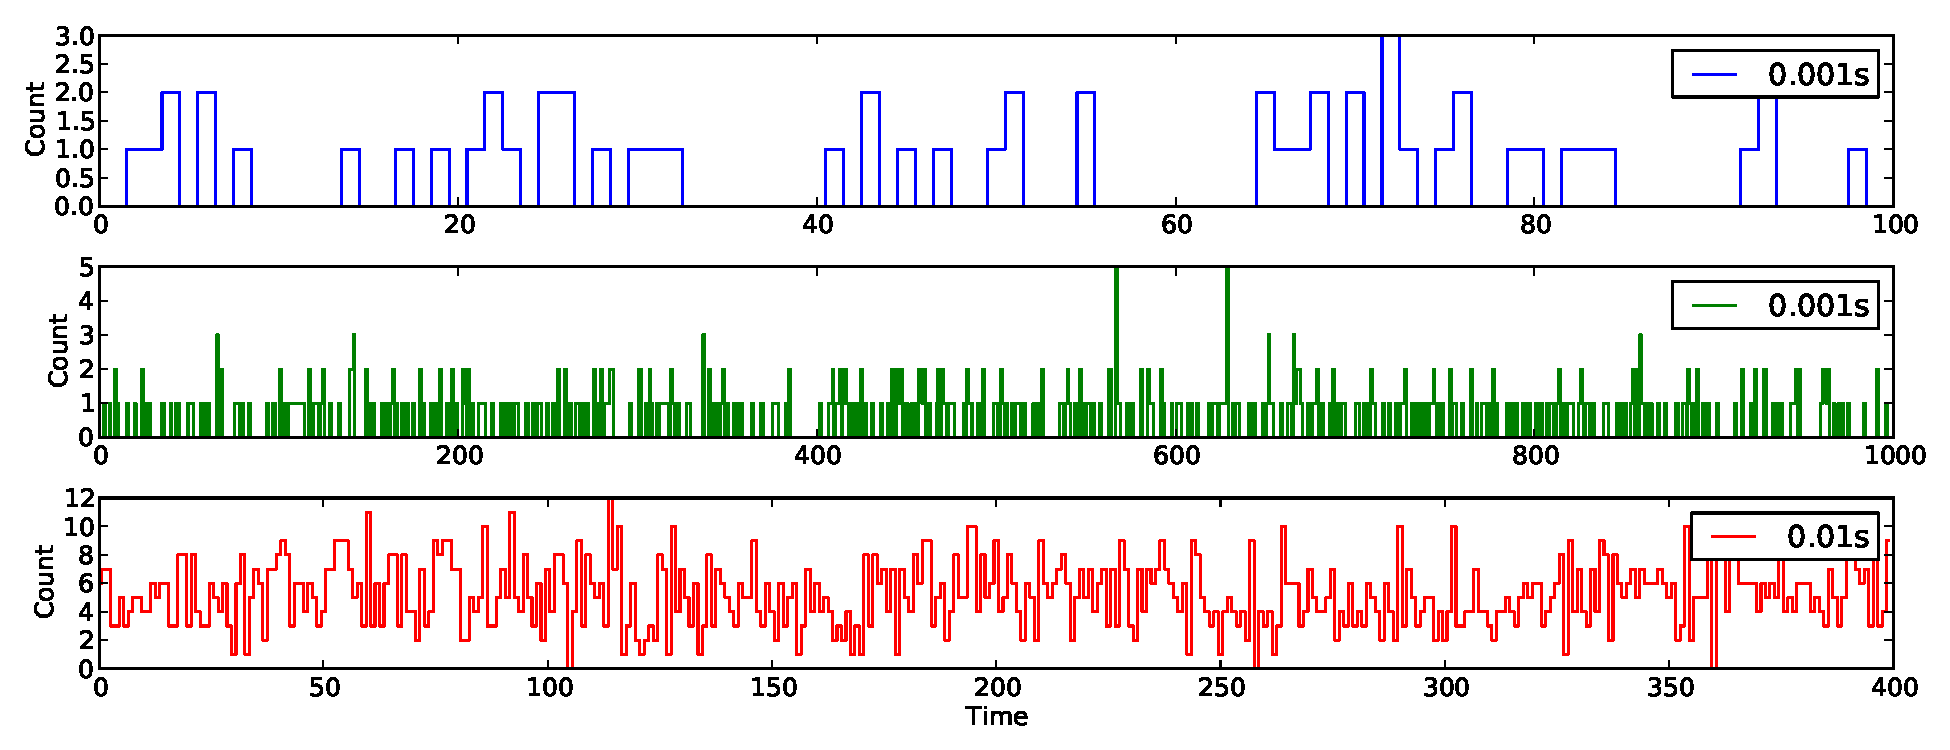
\includegraphics[angle=0,height=8cm,width=15.5cm]{graphs/dark_plots.pdf}
\caption{Count per Sample vs. Time graph for dark count  for three different set of data for Figure \ref{fig:diff_plot} and Figure \ref{fig:diff_hist}.}
\label{fig:dark_plot}
\end{figure}

\begin{figure}[H]
\centering
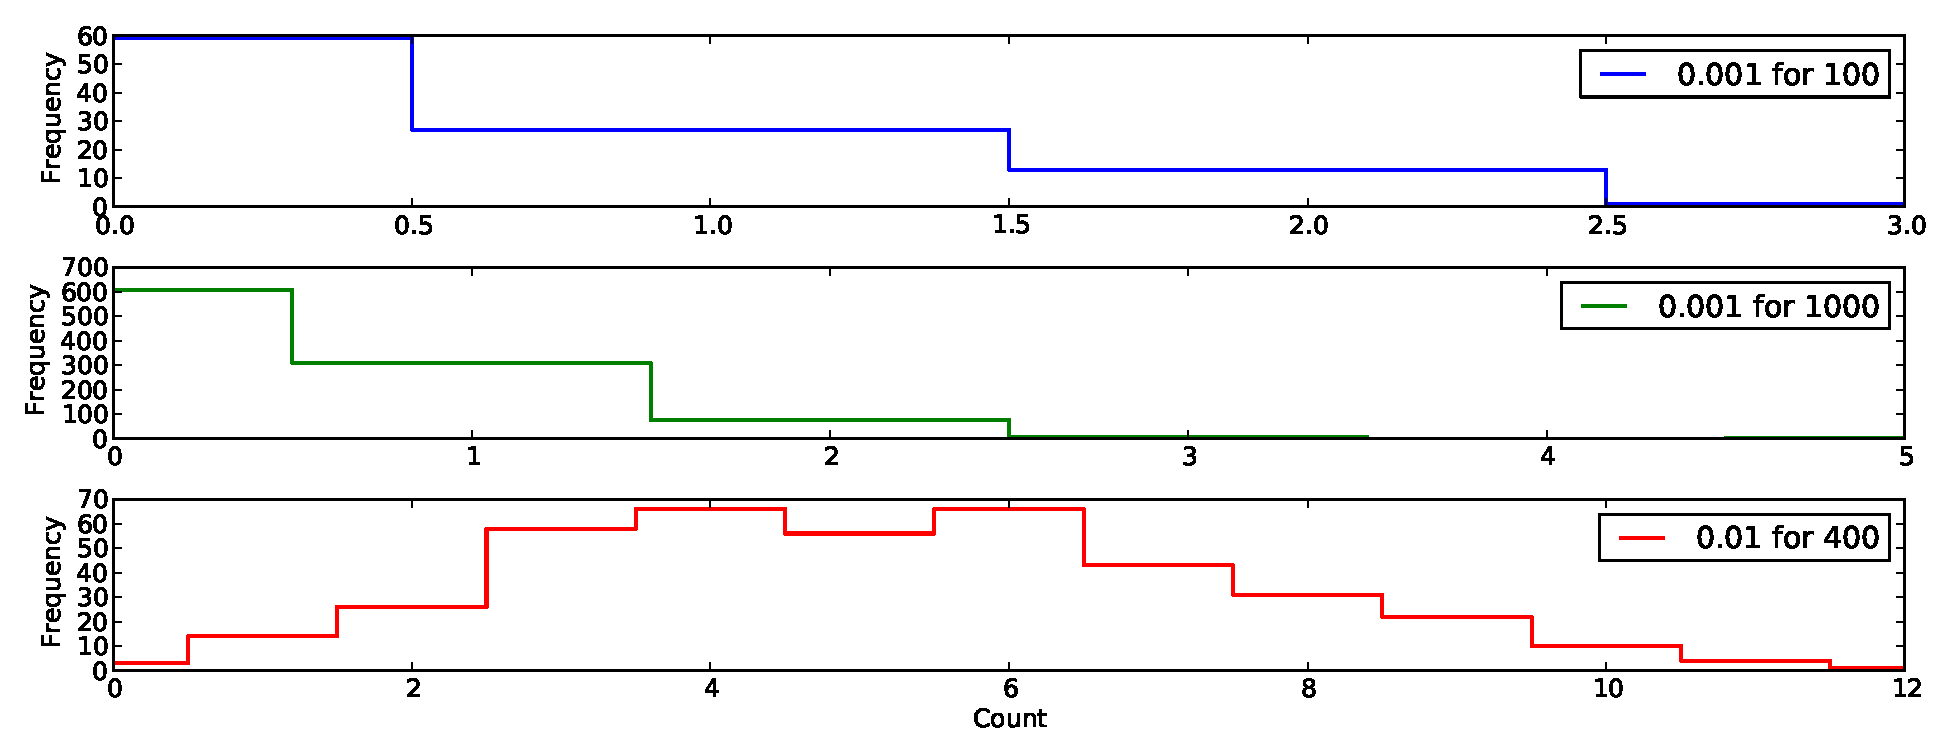
\includegraphics[angle=0,height=8cm,width=15.5cm]{graphs/dark_hist.pdf}
\caption{Histogram of data plotted in Figure \ref{fig:dark_plot}.}
\label{fig:dark_hist}
\end{figure}

%#################################################
what is the pattern. Does it look random? how do they effect it? what happen by changing sample size and time interval? should we take is under consideration or just ignore it? what is the source of all that noise

%%%%%%% ~~~~~~ count rate 
\subsection{Count rates of different sample}
\label{sec:countrate}

%%%%%%~~~~~~~ mean and variance
\subsection{Relationship between mean and variance}
\label{sec:meanandvariance}
How i got it. The equations required. 
%#################################################
%\begin{figure}[H]
%\centering
%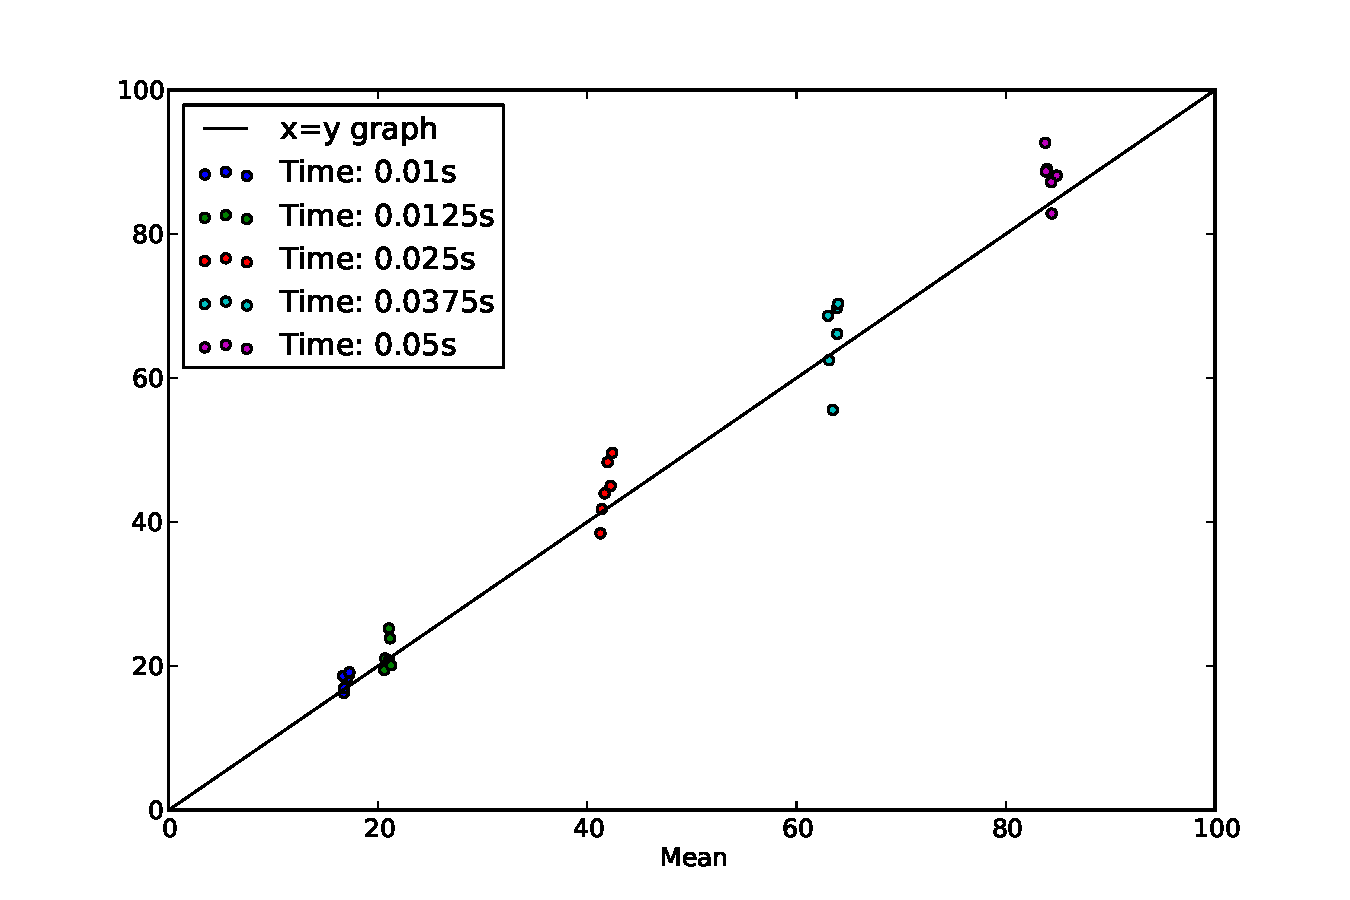
\includegraphics[angle=0,height=10cm,width=15.5cm]{graphs/Task7.pdf}
%\label{fig:task7}
%\end{figure}

\begin{figure}[H]
\centering
\centering
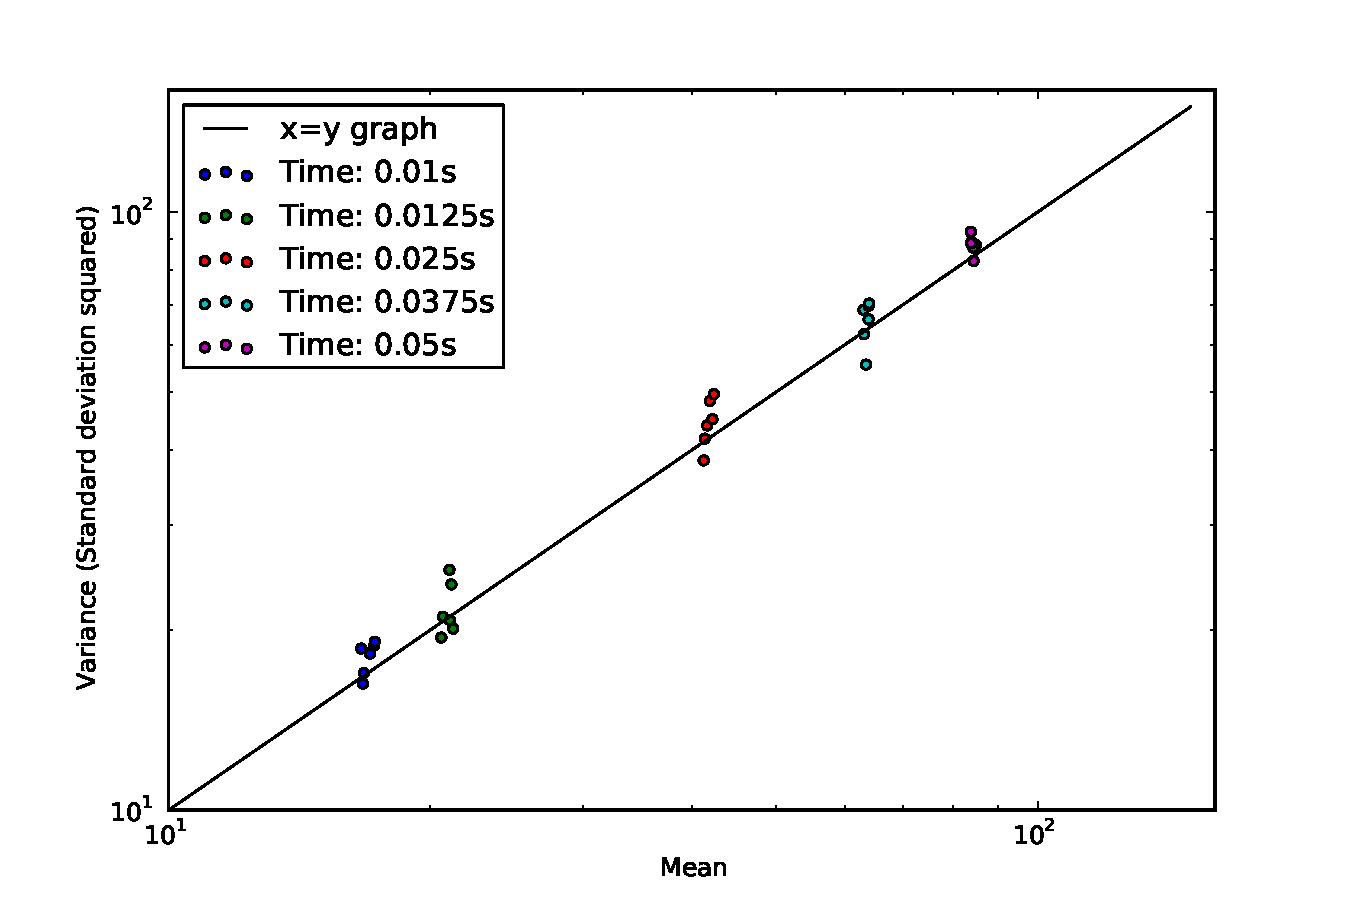
\includegraphics[angle=0,height=10cm,width=15.5cm]{graphs/Task7_log-log.pdf}
\label{fig:task7_log}
\caption{Mean vs. Variance (standard deviation squared) log-log graph. The sample size for all the data is 400. There are six sets of data for each of seven different time interval.}
\end{figure}
%#################################################
What does this represent/show.

%%%%%%% ~~~~~~theoritical prediction
\subsection{Compairing results with theotrical distribution}
\label{sec:theoritical}

%#################################################
\begin{figure}[H]
\centering
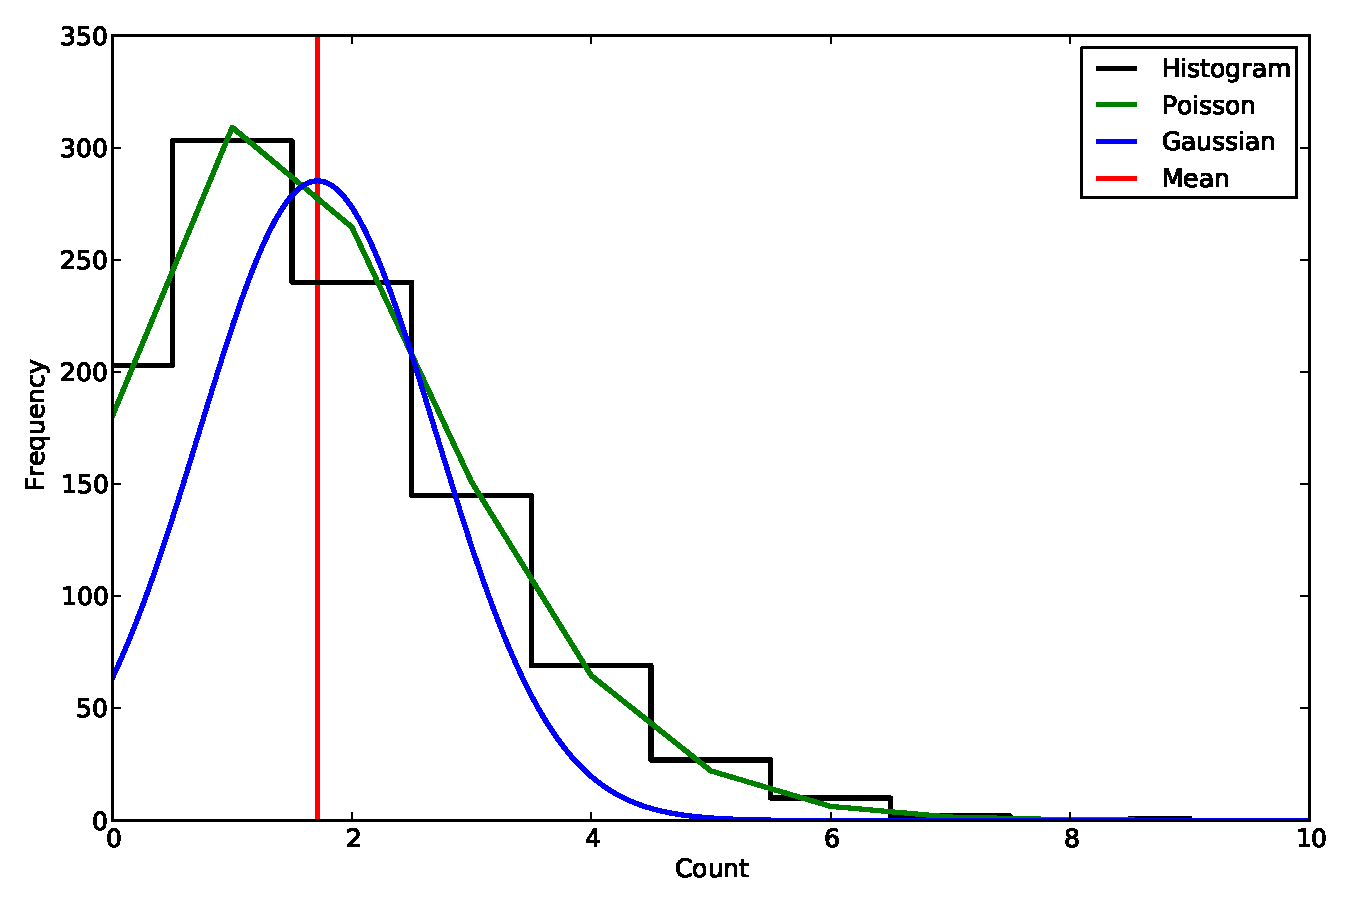
\includegraphics[angle=0,height=9cm,width=15.5cm]{graphs/Hist_distribution_small.pdf}
\caption{Histogram of one of the data with 1000 samples and time interval as 0.001. Here blues line is gaussian distribution, green is poisson distribution and red line indicated the mean value}
\label{fig:dark_plot}
\end{figure}

\begin{figure}[H]
\centering
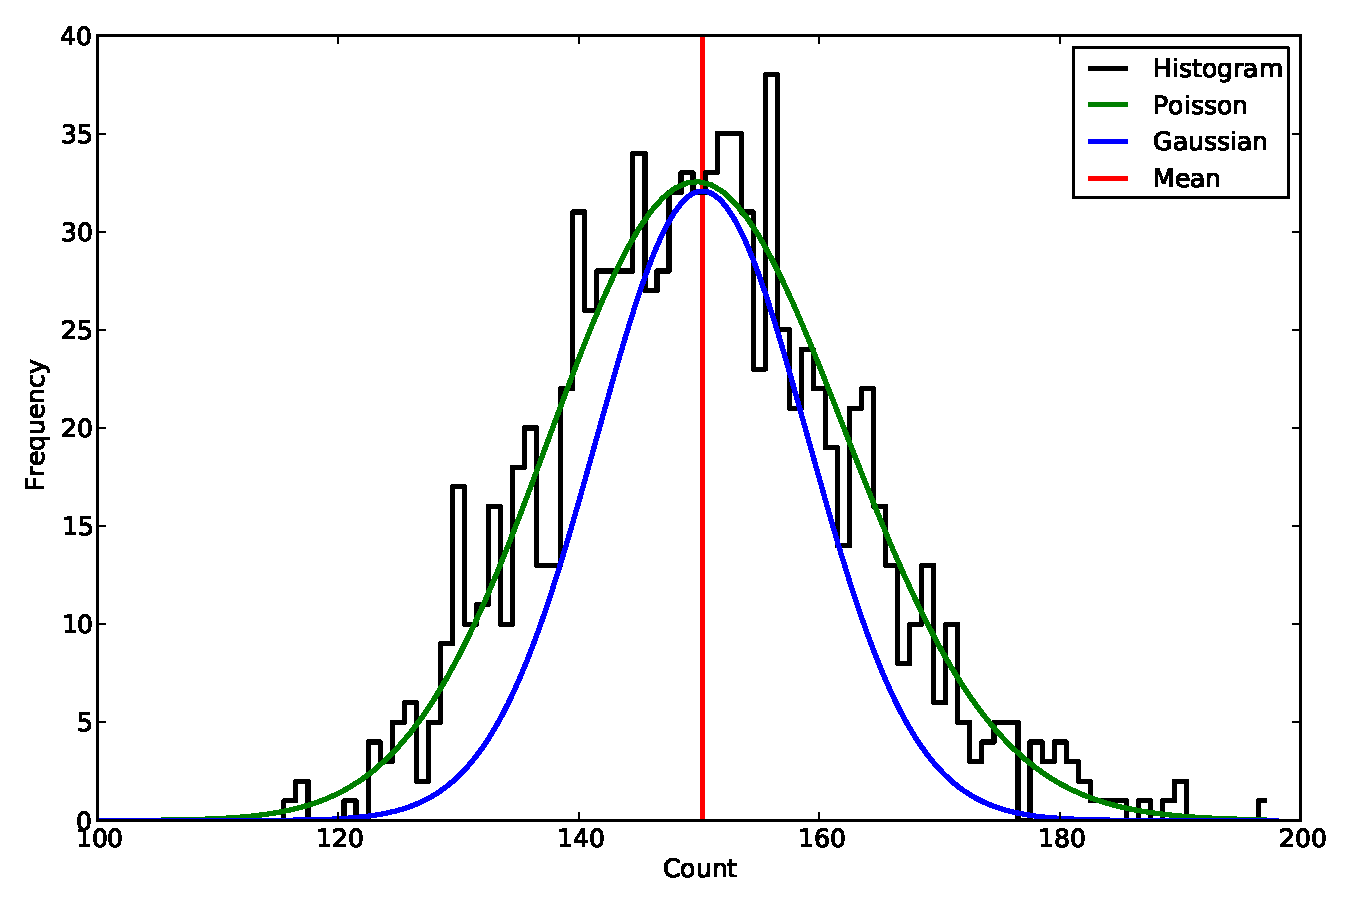
\includegraphics[angle=0,height=9cm,width=15.5cm]{graphs/Hist_distribution_big.pdf}
\caption{Histogram of one of the data with 1000 samples and time interval as 0.1. Here blues line is gaussian distribution, green is poisson distribution and red line indicated the mean value}
\label{fig:dark_hist}
\end{figure}

%#################################################

%%%%%%%% ~~~~~~~MOM and SDOM
\subsection{Exploring mean of mean and standard deviation of mean}
\label{sec:MOM_SDOM}



\section{Conclusion}
``I always thought something was fundamentally wrong with the universe'' \citep{adams1995hitchhiker}

\bibliographystyle{plain}
\bibliography{references}
\end{document}
